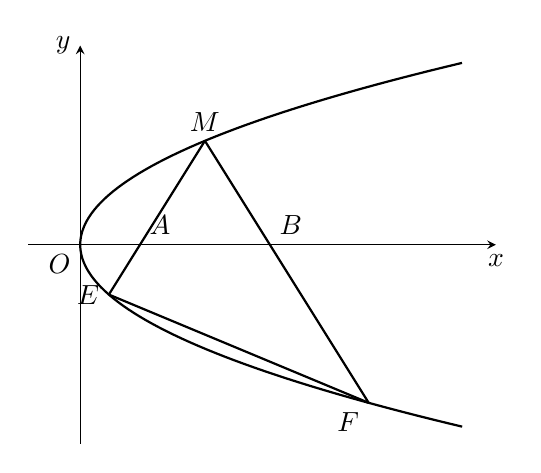
\begin{tikzpicture}[x=1.1cm,y=1.1cm,>=stealth]
  % 坐标轴
  \draw[->] (-0.6,0) -- (4.8,0) node[below] {$x$};
  \draw[->] (0,-2.3) -- (0,2.3) node[left] {$y$};
  \node[below left] at (0,0) {$O$};

  % 抛物线 y^2 = x (即 x = y^2)
  \draw[thick,domain=-2.1:2.1,samples=100] plot ({\x*\x},{\x});

  % 点 M(1.44, 1.2)
  \coordinate (M) at (1.44, 1.2);

  % 动弦 ME, MF
  % 设 k1 = 1.6, k2 = -1.6
  % yE = 1/1.6 - 1.2 = 0.625 - 1.2 = -0.575 => xE = 0.331
  % yF = -1/1.6 - 1.2 = -0.625 - 1.2 = -1.825 => xF = 3.331
  % xA = 1.44 - 1.2/1.6 = 1.44 - 0.75 = 0.69
  % xB = 1.44 + 0.75 = 2.19
  \coordinate (A) at (0.69, 0);
  \coordinate (B) at (2.19, 0);
  \coordinate (E) at (0.331, -0.575);
  \coordinate (F) at (3.331, -1.825);

  % 连线 ME, MF, EF
  \draw[thick] (M) -- (E);
  \draw[thick] (M) -- (F);
  \draw[thick] (E) -- (F);

  % 顶点与点标注
  \node[above] at (M) {$M$};
  \node[above right] at (A) {$A$};
  \node[above right] at (B) {$B$};
  \node[left] at (E) {$E$};
  \node[below left] at (F) {$F$};
\end{tikzpicture}
